\section{Direct kinematics}\label{sec:direct}
\subsection{Kinematic structure of the robot}\label{subsec:kine_struct}
The manipulator is a 6 DoF anthropomorphic arm with spherical wrist. The structure is
shown in Figure \ref{fig:kine_struct}.
\begin{figure}[H]
    \centering
    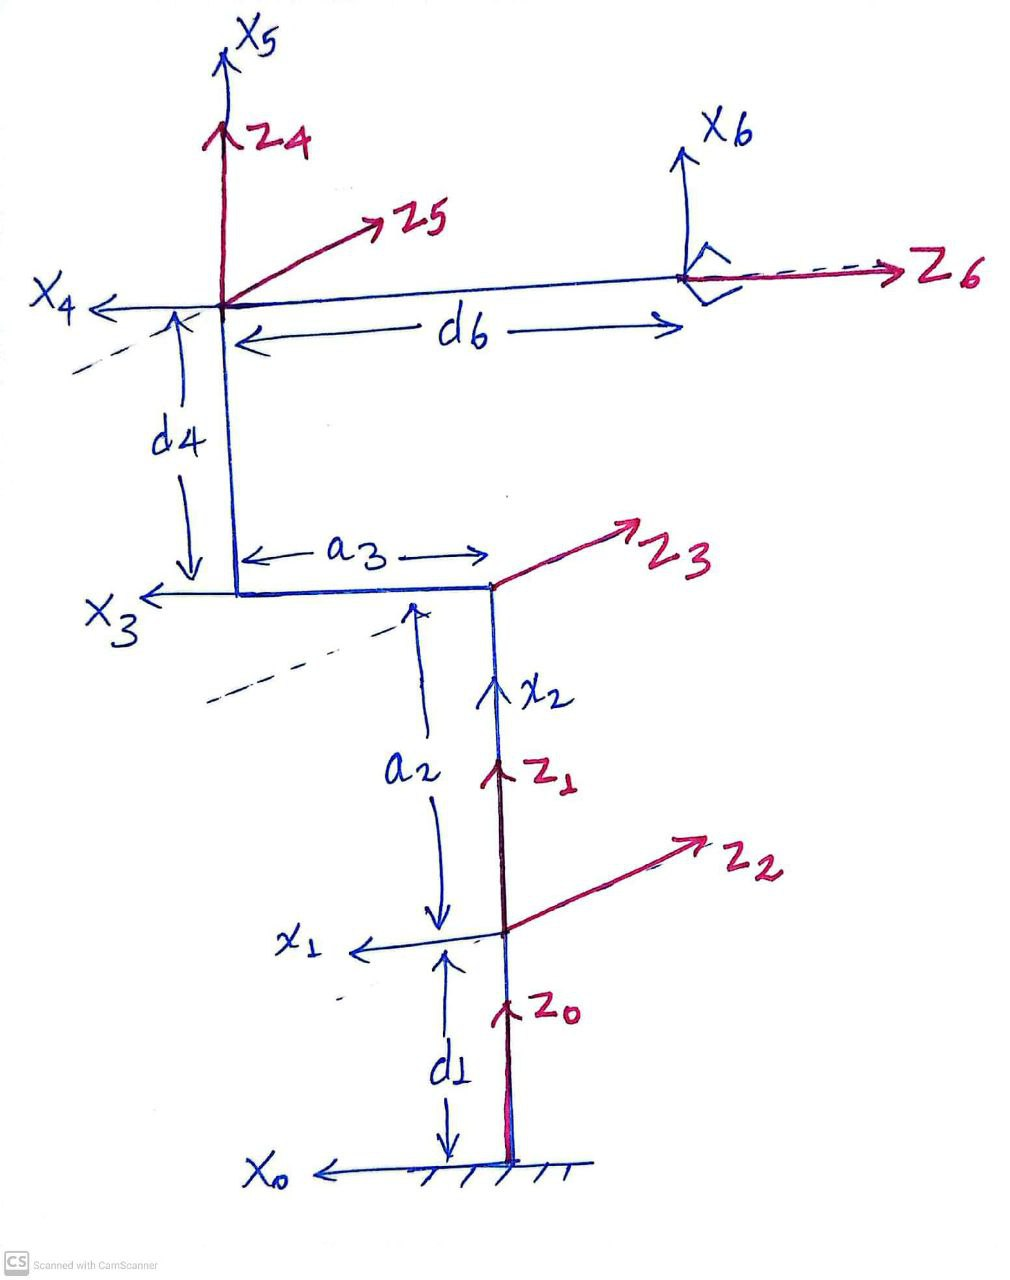
\includegraphics[width=0.5\textwidth]{images/kine_struct}
    \caption{Kinematic structure of the robot}
    \label{fig:kine_struct}
\end{figure}

% DH parameter
\subsection{Denavit-Hartenberg parameters}\label{subsec:dh}
We used the modified DH convention to perform the axis assignment and the result is shown
in Figure \ref{fig:kine_struct}.
The summary of the axis assignment is given below.
\begin{enumerate}
    \item Assign the $z_i$ axis along the $i^{th}$ axis of rotation.
          % Z axis assignment
          \begin{itemize}
              \item $i=1: z_1$ pointing up along axis 1 on the plane of the page.
              \item $i=2: z_2$ pointing into the page along axis 2.
              \item $i=3: z_3$ pointing into the page along axis 3.
              \item $i=4: z_4$ pointing up along axis 4 on the plane of the page.
              \item $i=5: z_5$ pointing into the page along axis 5.
              \item $i=6: z_6$ pointing to the right along axis 6 on the plane of the page.
          \end{itemize}
          % X axis assignment
    \item Find the common perpendiculars between the $z_{i-1}$ and $z_i$ axes.
          if those axes intersect the common perpendicular is defined along $z_{i-1}\times z_i$
    \item Define the $x_i$ axes. The axis $x_{i-1}$ coincides with the common perpendicular between
          axes $z_{i-1}$ and $z_i$ and points from $z_{i-1}$ to $z_i$.
\end{enumerate}
The DH parameters are defined as follows:
\begin{itemize}
    \item $a_{i-1}$: The distance between axes $z_{i-1}$ and $z_i$ measured along $x_{i-1}$
    \item $\alpha_{i-1}$: The angle between axes $z_{i-1}$ and $z_i$ measured around $x_{i-1}$
    \item $d_i$: The distance between axes $x_{i-1}$ and $x_i$ measured along $z_i$
    \item $\theta_i$: The angle between axes $x_{i-1}$ and $x_i$ measured around $z_i$
\end{itemize}
% DH table
\begin{table}[H]
    \centering
    \caption{DH parameters}
    \label{tab:dh}
    \begin{tabular}{|c|c|c|c|c|}
        \hline
        ${i}$ & $\alpha_{i-1}$ & $a_{i-1}$ & $d_i$ & $\theta_i$ \\\hline
        1     & 0              & 0         & $d_1$ & $\theta_1$ \\\hline
        2     & $-\pi/2$       & 0         & 0     & $\theta_2$ \\\hline
        3     & 0              & $a_2$     & 0     & $\theta_3$ \\\hline
        4     & $-\pi/2$       & $a_3$     & $d_4$ & $\theta_4$ \\\hline
        5     & $\pi/2$        & 0         & 0     & $\theta_5$ \\\hline
        6     & $-\pi/2$       & 0         & $d_6$ & $\theta_6$ \\
        \hline
    \end{tabular}
\end{table}
\subsection*{DH parameters verification}
The DH parameters have been verified using Peter Corke MATLAB robotics toolbox. The plot of the
robot at home position is shown in Figure \ref{fig:home}.
\begin{figure}[H]
    \centering
    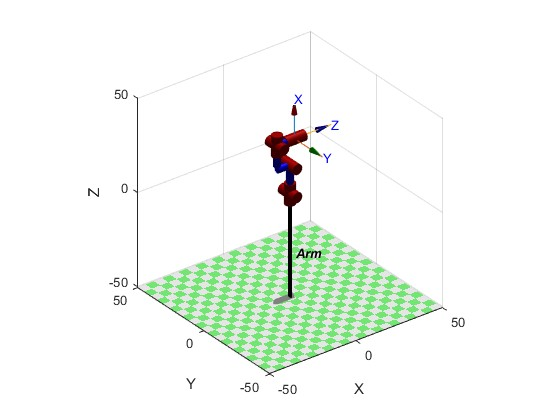
\includegraphics[width=0.5\textwidth]{images/dh_home}
    \caption{DH parameters verification}
    \label{fig:home}
\end{figure}

% Homogeneous transformation matrices
\subsection{Homogeneous transformation matrices}\label{subsec:hom_transf}
For the sake of simplicity, we define the following notations:
\begin{equation}\label{eq:simplicity}
    \begin{split}
        c_i&=cos(\theta_i)\\
        s_i&=sin(\theta_i)\\
        c_{ij}&=cos(\theta_i+\theta_j)\\
        s_{ij}&=sin(\theta_i+\theta_j)
    \end{split}
\end{equation}

% Insert dh frame assignmnet image
\begin{figure}[H]
    \centering
    \includegraphics[width=0.5\textwidth]{images/dh_frame}
    \caption{DH frame assignment}
    \label{fig:dh_frame}
\end{figure}

From the frame assignment shown in Figure \ref{fig:dh_frame},
the homogenous transformation matrix between frame $i$ and fram $i-1$ is given by:
\begin{equation} \label{eq:transf}
    {_i^{i-1}}T=Rot(x_{i-1},\alpha_{i-1})Trans(x_{i-1},a_{i-1})Rot(z_i,\theta_i)Trans(z_i,d_i)
\end{equation}

\begin{equation} \label{eq:hom_transf}
    {_i^{i-1}}T=\begin{bmatrix}
        c_i                  & -s_i                 & 0                 & a_{i-1}              \\
        s_i c_{\alpha_{i-1}} & c_i c_{\alpha_{i-1}} & -s_{\alpha_{i-1}} & -d_is_{\alpha_{i-1}} \\
        s_i s_{\alpha_{i-1}} & c_i s_{\alpha_{i-1}} & c_{\alpha_{i-1}}  & d_ic_{\alpha_{i-1}}  \\
        0                    & 0                    & 0                 & 1
    \end{bmatrix}
\end{equation}
Now, by substituting the DH parameters from Table \ref{tab:dh} into Equation \ref{eq:hom_transf},
let's solve the direct kinematics problem.

\begin{equation} \label{eq:hom_transf_prod}
    {_6^{0}}T=\prod_{i=1}^{6}{_i^{i-1}}T
\end{equation}

\begin{equation} \label{eq:T10}
    {_1^{0}}T=\begin{bmatrix}
        c_1 & -s_1 & 0 & 0   \\
        s_1 & c_1  & 0 & 0   \\
        0   & 0    & 1 & d_1 \\
        0   & 0    & 0 & 1
    \end{bmatrix}
\end{equation}

\begin{equation} \label{eq:T21}
    {_2^{1}}T=\begin{bmatrix}
        c_2  & -s_2 & 0 & 0 \\
        0    & 0    & 1 & 0 \\
        -s_2 & -c_2 & 0 & 0 \\
        0    & 0    & 0 & 1
    \end{bmatrix}
\end{equation}

\begin{equation} \label{eq:T20}
    {_2^{0}}T=\begin{bmatrix}
        c_1c_2 & -c_1s_2 & -s_1 & 0   \\
        c_2s_1 & -s_1s_2 & c_1  & 0   \\
        -s_2   & -c_2    & 0    & d_1 \\
        0      & 0       & 0    & 1
    \end{bmatrix}
\end{equation}

\begin{equation} \label{eq:T32}
    {_3^{2}}T=\begin{bmatrix}
        c_3 & -s_3 & 0 & a_2 \\
        s_3 & c_3  & 0 & 0   \\
        0   & 0    & 1 & 0   \\
        0   & 0    & 0 & 1
    \end{bmatrix}
\end{equation}

\begin{equation} \label{eq:T30}
    {_3^{0}}T=\begin{bmatrix}
        c_{23}c_1 & -s_{23}c_1 & -s_1 & a_2c_1c_2  \\
        c_{23}s_1 & -s_{23}s_1 & c_1  & a_2c_2s_1  \\
        -s_{23}   & -c_{23}    & 0    & d_1-a_2s_2 \\
        0         & 0          & 0    & 1
    \end{bmatrix}
\end{equation}

\begin{equation} \label{eq:T43}
    {_4^{3}}T=\begin{bmatrix}
        c_4  & -s_4 & 0 & a_3 \\
        0    & 0    & 1 & d_4 \\
        -s_4 & -c_4 & 0 & 0   \\
        0    & 0    & 0 & 1
    \end{bmatrix}
\end{equation}

\begin{equation} \label{eq:T40}
    {_4^{0}}T=\begin{bmatrix}
        s_1s_4+c_{23}c_1c_4 & c_4s_1-c_{23}c_1s_4  & -s_{23}c_1 & c_1\left(a_3c_{23}-d_4s_{23}+a_2c_2\right) \\
        c_{23}c_4s_1-c_1s_4 & -c_1c_4-c_{23}s_1s_4 & -s_{23}s_1 & s_1\left(a_3c_{23}-d_4s_{23}+a_2c_2\right) \\
        -s_{23}c_4          & s_{23}s_4            & -c_{23}    & d_1-d_4c_{23}-a_3s_{23}-a_2s_2             \\
        0                   & 0                    & 0          & 1
    \end{bmatrix}
\end{equation}

\begin{equation} \label{eq:T54}
    {_5^{4}}T=\begin{bmatrix}
        c_5 & -s_5 & 0  & 0 \\
        0   & 0    & -1 & 0 \\
        s_5 & c_5  & 0  & 0 \\
        0   & 0    & 0  & 1
    \end{bmatrix}
\end{equation}

\begin{equation} \label{eq:T50}
    {_5^{0}}T=\begin{bmatrix}
        % 1st row
        \begin{aligned}
             & c_5\left(s_1s_4 + c_{23}c_1c_4\right) \\
             & -s_{23}c_1s_5
        \end{aligned}  &
        \begin{aligned}
             & -s_5\left(s_1s_4 + c_{23}c_1c_4\right) \\
             & -s_{23}c_1c_5
        \end{aligned} & c_{23}c_1s_4 - c_4s_1    &
        c_1\left(a_3c_{23} - d_4s_{23} + a_2c_2\right)                                                                                                       \\\\
        % 2nd row
        \begin{aligned}
             & -c_5\left(c_1s_4 - c_{23}c_4s_1\right) \\
             & - s_{23}s_1s_5
        \end{aligned} &
        \begin{aligned}
             & s_5\left(c_1s_4 - c_{23}c_4s_1\right) \\
             & - s_{23}c_5s_1
        \end{aligned}  & c_1c_4 + c_{23}s_1s_4    & s_1(a_3c_{23} - d_4s_{23} + a_2c_2)                                                                      \\\\
        % 3rd row
        - c_{23}s_5 - s_{23}c_4c_5                   & s_{23}c_4s_5 - c_{23}c_5 & -s_{23}s_4                          & d_1 - d_4c_{23} - a_3s_{23} - a_2s_2 \\\\
        0                                            & 0                        & 0                                   & 1
    \end{bmatrix}
\end{equation}

\begin{equation} \label{eq:T65}
    {_6^{5}}T=\begin{bmatrix}
        c_6  & -s_6 & 0 & 0   \\
        0    & 0    & 1 & d_6 \\
        -s_6 & -c_6 & 0 & 0   \\
        0    & 0    & 0 & 1
    \end{bmatrix}
\end{equation}

% Direct kinematics
\begin{equation} \label{eq:T60}
    \setlength{\arraycolsep}{1pt}
    {_6^{0}}T=\begin{bmatrix}
        % 1st row
        \begin{aligned}
             & c_5c_6\left(s_1s_4 + c_{23}c_1c_4\right)\\
             & -s_{23}c_1c_6s_5 \\
             & +s_6\left(c_4s_1 - c_{23}c_1s_4\right)
        \end{aligned}   &
        \begin{aligned}
             & -c_5s_6\left(s_1s_4 + c_{23}c_1c_4\right) \\
             &+ s_{23}c_1s_5s_6 \\
             & +c_6\left(c_4s_1 - c_{23}c_1s_4\right)
        \end{aligned} &
        \begin{aligned}
             & -s_1s_4s_5 \\
             &- c_{23}c_1c_4s_5 \\
             & -s_{23}c_1c_5
        \end{aligned}                              &
        \begin{aligned}
             & c_1\left(a_3c_{23} - d_4s_{23} + a_2c_2\right)                        \\
             & -d_6s_5\left(s_1s_4 + c_{23}c_1c_4\right) \\
             &+ -d_6s_{23}c_1c_5
        \end{aligned}              \\\\
        % 2nd row
        \begin{aligned}
             & -c_5c_6\left(c_1s_4 - c_{23}c_4s_1\right) \\
             &- s_{23}c_6s_1s_5 \\
             & -s_6\left(c_1c_4 + c_{23}s_1s_4\right)
        \end{aligned} &
        \begin{aligned}
             & s_6c_5\left(c_1s_4 - c_{23}c_4s_1\right) \\
             &+ s_{23}s_1s_5s_6 \\
             & -c_6\left(c_1c_4 + c_{23}s_1s_4\right)
        \end{aligned}  &
        \begin{aligned}
             & c_1s_4s_5 \\
             &- c_{23}c_4s_1s_5 \\
             & -s_{23}c_5s_1
        \end{aligned}                               &
        \begin{aligned}
             & s_1\left(a_3c_{23} - d_4s_{23} + a_2c_2\right)                        \\
             & +d_6s_5\left(c_1s_4 - c_{23}c_4s_1\right) \\
             &- d_6s_{23}c_5s_1
        \end{aligned}              \\\\
        % 3rd row
        \begin{aligned}
             & -c_6c_{23}s_5 \\
             &- s_{23}c_4c_5c_6 \\
             & +s_{23}s_4s_6
        \end{aligned}                           &
        \begin{aligned}
             & c_{23}s_5s_6 \\
             &+ s_{23}c_4c_5s_6 \\
             & +s_{23}c_6s_4
        \end{aligned}                            &
        \begin{aligned}
             & s_{23}c_4s_5 \\
             & -c_{23}c_5
        \end{aligned}                                                        &
        \begin{aligned}
             & d_1 - d_4*c_{23} - a_3*s_{23} \\
             & - a_2s_2 -d_6c_{23}c_5 \\
             & + d_6s_{23}c_4s_5
        \end{aligned}                                          \\\\
        0                                                                         & 0 & 0 & 1
    \end{bmatrix}
\end{equation}

